\documentclass{article}
  % Packages and settings
  \usepackage{fontspec}
    \setmainfont{Charis SIL}
  \usepackage{listings}
    \lstset{basicstyle=\ttfamily,
            breaklines=true,
            language=Python}
  \usepackage{graphicx}
    \graphicspath{{figures/}}

  % Document information
  \title{Homework 7}
  \author{Joshua McNeill}
  \date{\today}

  % New commands
  \newcommand{\orth}[1]{$\langle$#1$\rangle$}
  \newcommand{\lexi}[1]{\textit{#1}}

\begin{document}
  \maketitle
  From the UD\_French-GSD corpus, I looked at the errors in parsing the following sentence:
  \begin{itemize}
    \item[] C'est de cette façon que des conditions socio-économiques radicalement nouvelles ( néolibéralisme ) ont été imposées durant les années 1980 à 1990. \\
    \item[] `It's in this way that the radically new socioeconomic conditions (neoliberalism) had been imposed during the 1980s to the 1990s.'
  \end{itemize}
  The errors themselves looked like the following:
  \lstinputlisting[lastline=13]{errors.txt}
  The tree created with these errors can be seen in Figure \ref{fig:spacy}, which compares to the gold standard in Figure \ref{fig:grew}.
  To start, spaCy made \lexi{radicalement} the nominal subject of \lexi{conditions} even though the former is an adverb and the latter a noun.
  The Grew version instead makes \lexi{radicalement} an adverb that modifies the adjective \lexi{nouvelles}, which can be glossed as `radically new.'
  Likewise, \lexi{radicalement} was made the nominal subject of the passive verbal form \lexi{imposées}, which is clearly not possible.
  Again, the Grew version correctly made \lexi{conditions} the subject.

  In fact, the errors usually involved either \lexi{radicalement} or \lexi{imposées}.
  For instance, the complementizer \lexi{que} was made the dependent of \lexi{radicalement}, though it should be the dependent of \lexi{imposées}.
  \lexi{Radicalement} was also put into an open clausal complement relation with \lexi{nouvelles}, though neither are verbs as would be needed.
  This was perhaps an issue with the parenthetical \lexi{néoliberalisme} that comes right after to clarify what the subject is describing.
  spaCy did at least treat \lexi{néoliberalisme} correctly as a parenthetical, but it should have been the dependent of \lexi{conditions}, as the Grew version parsed it.

  What ultimately seems to be an issue is when the word order is not particularly regular.
  In the sentence analyzed, there are two adjectives describing \lexi{conditions}: \lexi{socio-économiques} and \lexi{nouvelles}.
  However, \lexi{radicalement} is inserted between them because it only modifies the latter, which appears to be a problem for the parser.
  Similarly, the parser has trouble with the parenthetical \lexi{néoliberalisme}.
  \begin{figure}[tbh]
    \caption{spaCy dependency tree}
    \label{fig:spacy}
    \centering
    \includegraphics[scale=0.61]{dep_tree_spacy.pdf}
  \end{figure}
  \begin{figure}[tbh]
    \caption{Grew dependency tree}
    \label{fig:grew}
    \centering
    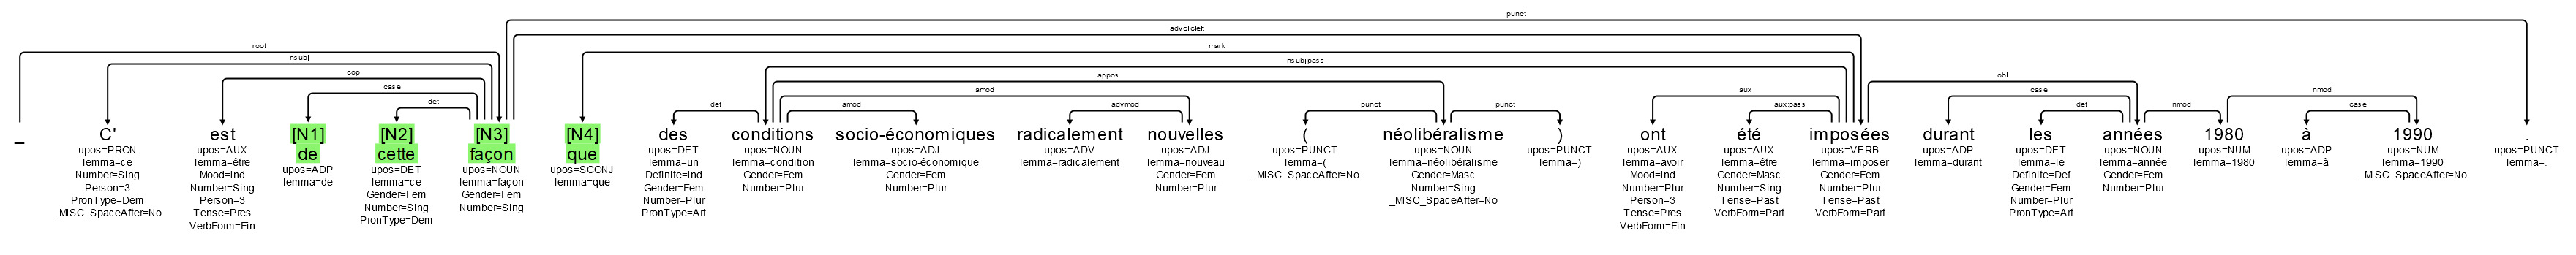
\includegraphics[scale=0.095]{dep_tree_grew.jpg}
  \end{figure}
\end{document}
